\documentclass{ltjsarticle}

\usepackage{graphics}
\begin{document}

\title{雪に関する音楽}
\author{細田真道}
\date{2018年12月17日}
\maketitle

\tableofcontents
\clearpage

\section{童謡}

雪やゆきだるまに関する童謡を探してみました。

\subsection{雪}

雪に関する童謡としては非常に有名ですね。
おそらくほとんどの方がご存じなのではないでしょうか。
題名はそのままストレートに「雪」、
「尋常小学校唱歌」第二学年用(明治44年/ 1911年)が初出だそうです。
冒頭部分を以下に示します。

{%
\parindent 0pt
\noindent
\ifx\preLilyPondExample \undefined
\else
  \expandafter\preLilyPondExample
\fi
\def\lilypondbook{}%
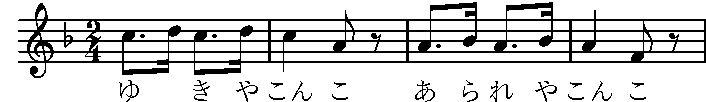
\includegraphics{/mnt/c/Users/haru/working/zenn-test-2/1c/lily-512fd6ec-1}%
% eof
%
\ifx\postLilyPondExample \undefined
\else
  \expandafter\postLilyPondExample
\fi
}

\subsection{雪達磨}

ゆきだるまに関する童謡を探してみたところ、こんなものを見つけました。
題名は「雪達磨」、
「新訂尋常小学唱歌」第一学年用(昭和7年/ 1932年)に掲載されているそうです。
冒頭部分を以下に示します。

{%
\parindent 0pt
\noindent
\ifx\preLilyPondExample \undefined
\else
  \expandafter\preLilyPondExample
\fi
\def\lilypondbook{}%
\includegraphics{/mnt/c/Users/haru/working/zenn-test-2/6b/lily-f6bf65f3-1}%
% eof
%
\ifx\postLilyPondExample \undefined
\else
  \expandafter\postLilyPondExample
\fi
}

\end{document}

